\section{Camera Calibration}
\label{sec::51_cc}
As described in section \ref{sec::324_ip}, in order for the stereo block matching algorithm to work properly (equation \ref{eq::324_sad}), it is required to calibrate the cameras. We therefore chose to use a chess-board calibration pattern, see figure \ref{fig::51_calib}. The used calibration pattern has width of $W=8$, and a height of $H=6$, where each square has a size of $a=22.5\,\text{mm}$ (equation \ref{eq::324_square_size}). We took a total of $N=60$ images of the calibration pattern for varying orientations and translations with respect to the camera, which results in a total of $W\times H\times N = 2880$ points for the calibration. 
\begin{figure}[h]
	\centering
	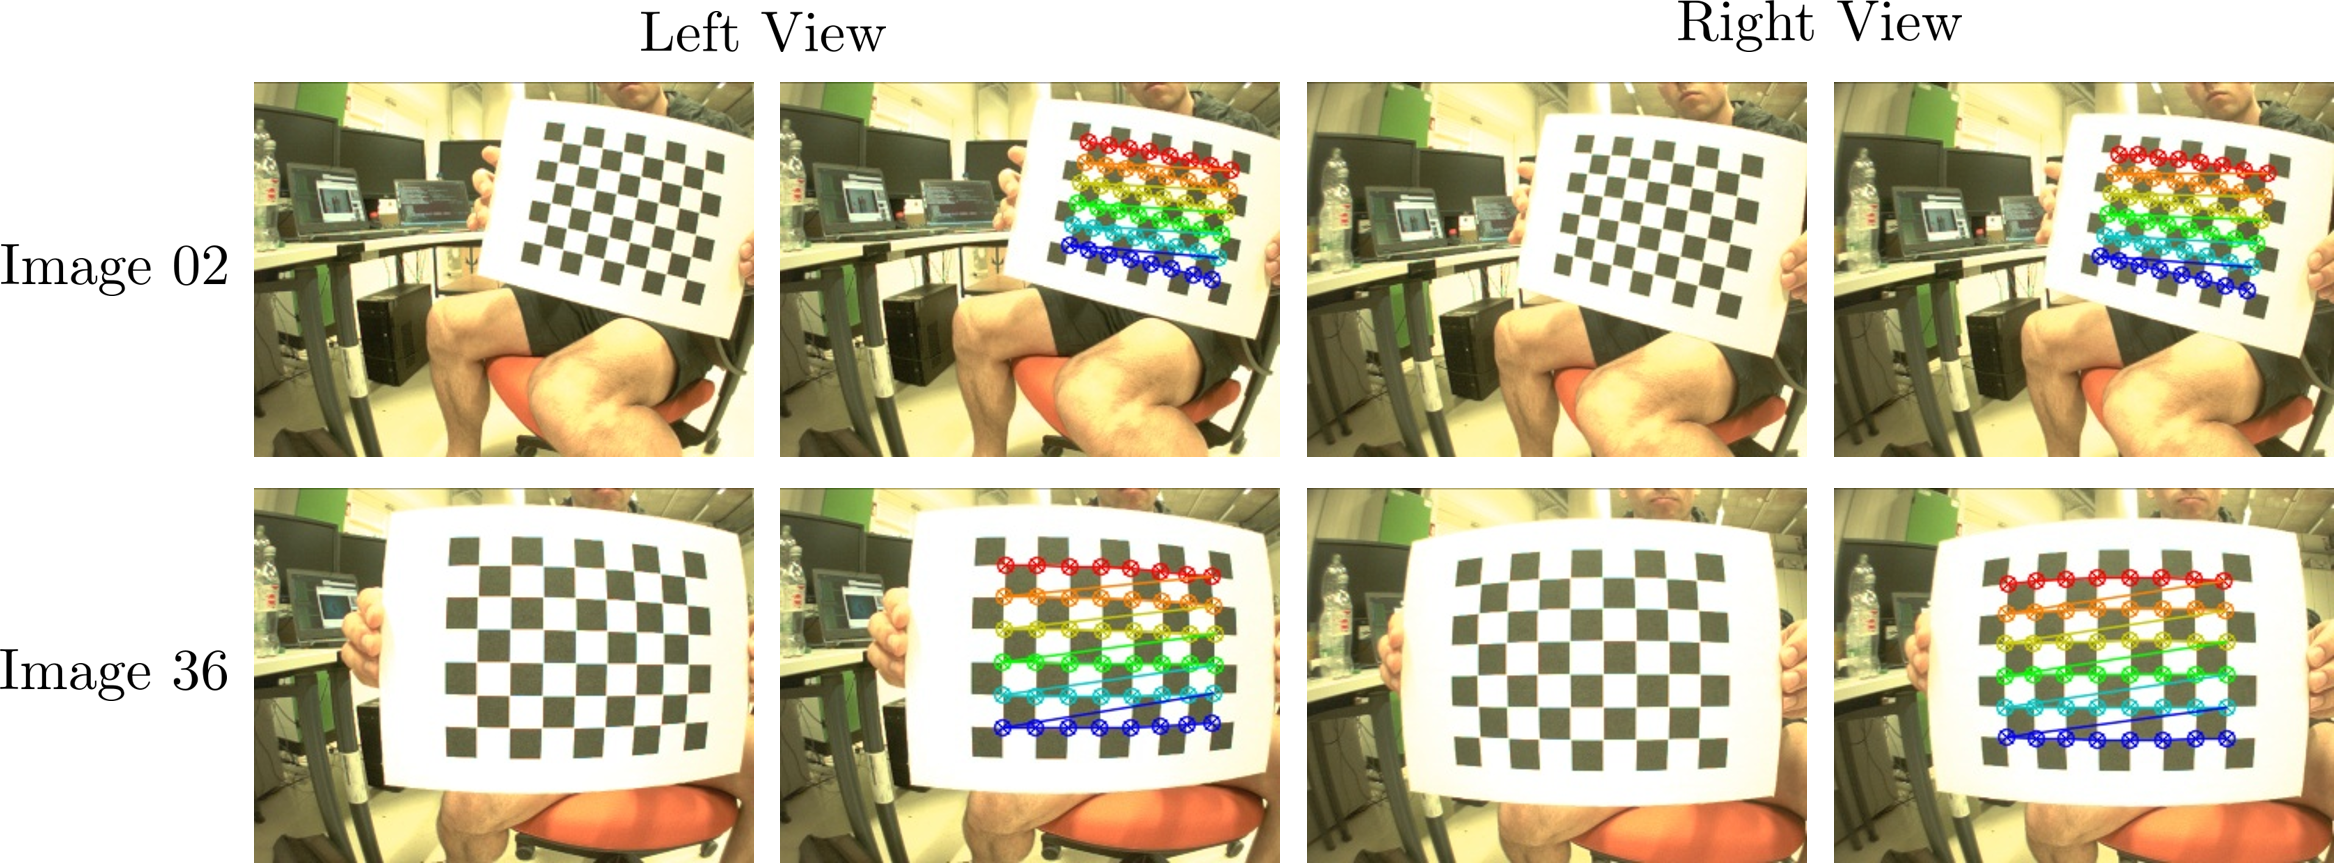
\includegraphics[scale=.28]{chapters/05_experiments/01_camera_calibration/calib.png}
	\caption{Exemplary left and right camera views of the calibration pattern as acquired during the calibration process. The colorful points indicate the detected corners in the image plane. Refer to figure \ref{fig::324_distortion} for the theory.}
	\label{fig::51_calib}
\end{figure}
oAs the resulting mean squared re-projection error $\Delta \bar{x} = 1/(WHN)\sum_0^{WHN} \Delta x$ (equation \ref{eq::324_reprojection}), we obtained $\Delta \bar{x}_l = 0.26\, \text{pixel}$, and $\Delta \bar{x}_r = 0.25\,\text{pixel}$, for the left, and the right camera, respectively. According to equations \ref{eq::324_focal_intrinsics}, \ref{eq::324_x_dist}, and \ref{eq::324_y_dist}, we therefore determined the camera intrinsic parameters as listed in table \ref{tab::51_intrinsics}.
\begin{table}
	\centering
	\begin{tabular}{lll}
		Intrinsic Parameter & Left Camera & Right Camera\\
		\hline
		$f_x$ & $\quad2.36\cdot10^2$ & $\quad2.32\cdot10^2$ \\
		$f_y$ & $\quad2.37\cdot10^2$ & $\quad2.32\cdot10^2$ \\
		$c_x$ & $\quad1.63\cdot10^2$ & $\quad1.86\cdot10^2$ \\
		$c_y$ & $\quad1.11\cdot10^2$ & $\quad1.30\cdot10^2$ \\
		$k_1$ & $-4.54\cdot10^{-1}$ & $-4.58\cdot10^{-1}$ \\
		$k_2$ & $\quad2.90\cdot10^{-1}$  & $\quad3.18\cdot10^{-1}$  \\
		$k_3$ & $-1.21\cdot10^{-1}$ & $-1.48\cdot10^{-1}$ \\
		$p_1$ & $-2.73\cdot10^{-3}$ & $\quad3.02\cdot10^{-4}$  \\
		$p_2$ & $\quad2.16\cdot10^{-4}$  & $\quad7.63\cdot10^{-4}$		
	\end{tabular}
	\caption{Intrinsic parameters of single cameras. These parameters can be found as YAML file on GitHub (\href{https://github.com/mhubii/nmpc_pattern_generator/tree/master/libs/io_module}{link}).\label{tab::51_intrinsics}}
\end{table}
Then given the calibration of each single camera, we computed the rectification transforms $\bm{R}$, and the projection matrices $\bm{P}$ in the rectified coordinate system for each camera \ref{tab::51_extrinsics}.
\begin{table}
	\centering
	\begin{tabular}{lll}
		Camera & Extrinsic Parameter & \\ 
		\hline
		&& \\
		\multirow{5}{*}{Left} & $\bm{R}$              & $\begin{pmatrix}
		\quad9.93\cdot10^{-1} & -2.65\cdot10^{-3}     & \quad1.14\cdot10^{-1} \\ 
		\quad5.41\cdot10^{-1} & \quad1.00\cdot10^{0}  & -2.39\cdot10^{-2} \\
		-1.14\cdot10^{-1}     & \quad2.43\cdot10^{-2} & \quad9.93\cdot10^{-1}
		\end{pmatrix}$ \\&&\\
		                      & $\bm{P}$              & $\begin{pmatrix}
        2.34\cdot10^{2} & 0.00     & 1.88\cdot10^{2} & 0.00 \\ 
        0.00 & 2.34\cdot10^{2}  & 4.87\cdot10^{1} & 0.00 \\
        0.00    & 0.00 & 1.00 & 0.00
        \end{pmatrix}$ \\
        &&\\
        \multirow{5}{*}{Right} & $\bm{R}$              & $\begin{pmatrix}
        \quad9.95\cdot10^{-1} & -2.30\cdot10^{-2}     & \quad9.93\cdot10^{-2} \\ 
        \quad2.07\cdot10^{-2} & \quad1.00\cdot10^{0}  & \quad2.38\cdot10^{-2} \\
        -9.98\cdot10^{-2}     & -2.16\cdot10^{-2} & \quad9.95\cdot10^{-1}
        \end{pmatrix}$ \\&&\\
        & $\bm{P}$              & $\begin{pmatrix}
        2.34\cdot10^{2} & 0.00     & 1.88\cdot10^{2} & -1.60\cdot10^1 \\ 
        0.00 & 2.34\cdot10^{2}  & 4.88\cdot10^{1} & 0.00 \\
        0.00    & 0.00 & 1.00 & 0.00
        \end{pmatrix}$ \\
	\end{tabular}
	\caption{Rectification transform $\bm{R}$, and projection matrices $\bm{P}$, for the left, and the right camera, respectively. These parameters can be found as YAML file on GitHub (\href{https://github.com/mhubii/nmpc_pattern_generator/blob/master/libs/io_module/cam_stereo.yaml}{link}). \label{tab::51_extrinsics}}
\end{table}
Exemplary rectified images, which rely on the matrices of table \ref{tab::51_extrinsics}, are shown in figure \ref{fig::51_rect}. Since there is a slight rotation of the calibration pattern, it is not obvious that the images got rectified well. Therefore, the same images are shown in figure \ref{fig::51_rect_line}, but slightly rotated such that the calibration pattern aligns horizontally. The blue line therein indicates that in contrast to the original image, straight lines now appear straight across both images, which is crucial for the block matching algorithm in the next section - Depth Map Parameter Tuning.
\begin{figure}[h]
	\centering
	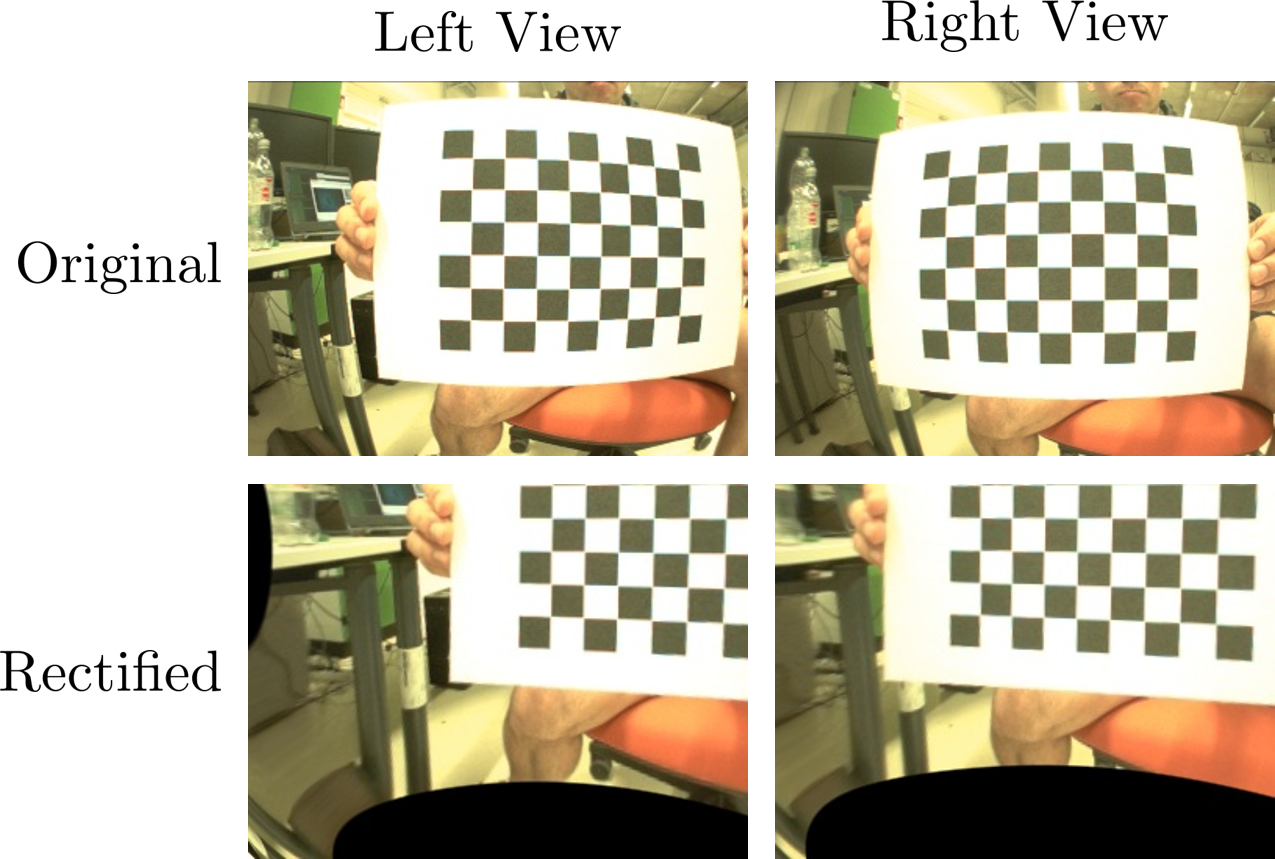
\includegraphics[scale=.28]{chapters/05_experiments/01_camera_calibration/rect.png}
	\caption{Rectified and original view of the stereo camera. Due to a slight rotation of the calibration pattern, it does not immediately become clear that the image got rectified correctly, see figure \ref{fig::51_rect_line}. Refer to figure \ref{fig::324_rectified} for the theory.}
	\label{fig::51_rect}
\end{figure}
\begin{figure}[h]
	\centering
	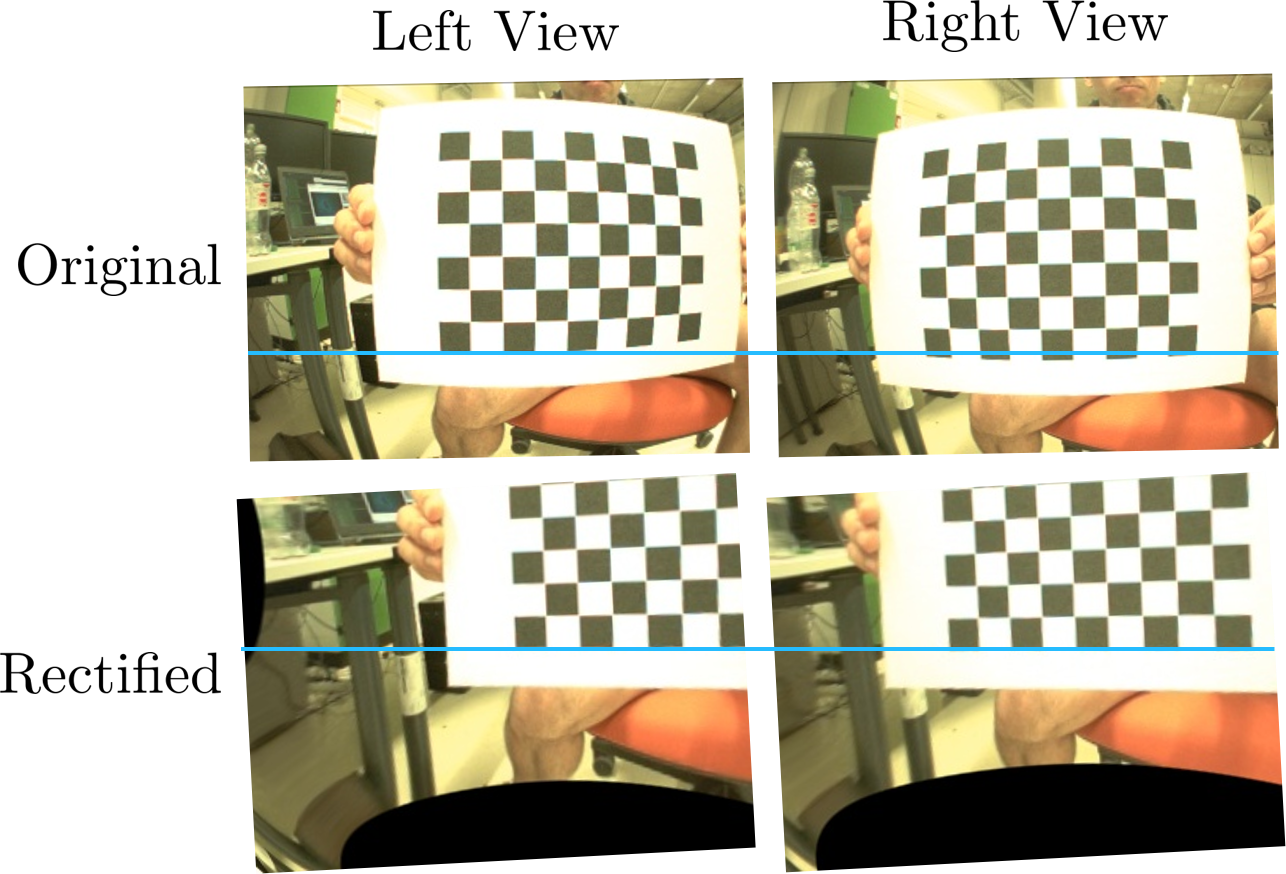
\includegraphics[scale=.28]{chapters/05_experiments/01_camera_calibration/rect_line.png}
	\caption{Same images as shown in figure \ref{fig::51_rect}, but rotated such that the blue line indicates that straight lines are now indeed straight. Please note that the blue lines do not correspond to the epipolar lines, but to rotated versions of them.}
	\label{fig::51_rect_line}
\end{figure}
